%!TEX program = xelatex
\documentclass[12pt,hyperref,a4paper,UTF8]{ctexart}
\usepackage{UIBEReport}

%% ─── 超链接颜色与定义 ─────────────────────────────────────────
\definecolor{winered}{rgb}{0.5,0,0}
\hypersetup{
  colorlinks = true,
  linkcolor  = {winered},
  citecolor  = {winered},
  urlcolor   = {winered},
}

%% ─── 额外宏包 ──────────────────────────────────────────────
\usepackage{siunitx}
\usepackage{rotating}
\usepackage{dcolumn}

%% ─── 标题页信息 ────────────────────────────────────────────
\title{\songti\bfseries\zihao{2} 国家新一代人工智能创新发展试验区政策对企业研发投入的影响：\\来自多期双重差分的证据\thanks{本文利用A股上市公司2013—2025年面板数据，采用多期双重差分法评估中国AI试验区政策对企业创新投入的影响。感谢匿名审稿人的宝贵意见。文责自负。作者简介：陈沫樵，中国金融学院鸿儒2401班硕士研究生，学号：202442087。}}
\author{\kaishu\zihao{4} 陈沫樵}
\date{}

\newtoks\header
\header{AI试验区政策与企业研发投入}

\newtoks\entitle
\newtoks\enauthor
\newtoks\eninstitute
\newtoks\enabstract
\newtoks\enkeywords

\entitle{National AI Innovation Zones and Corporate R\&D Investment:\\
Evidence from Staggered Difference-in-Differences}
\enauthor{Mochiao Chen}
\eninstitute{UIBE}
\enabstract{%
This paper evaluates the effects of China's National AI Innovation Zone (\textit{Guojia Xinshidai Rengong Zhineng Chuangxin Fazhan Shiyanqu}) policy on corporate R\&D investment using a staggered difference-in-differences design. Exploiting four designation waves (2019--2022) across 4,875 A-share listed firms over 2013--2025, we find that the aggregate two-way fixed effects estimate is statistically insignificant (coefficient~= 0.04~pp, \textit{t}~= 1.38), yet this average conceals substantial heterogeneity. Cohort-by-cohort decomposition reveals that the 2019 and 2021 designation cohorts---smaller, more selectively targeted batches---generate significant R\&D increases of 0.23 and 0.13 percentage points respectively, while the 2020 mass-rollout cohort (comprising 51\% of all treated firms) produces no effect, diluting the aggregate estimate. Industry-level heterogeneity shows significant effects only among high-AI-exposure firms (\textit{t}~= 3.74, significant at 1\%), with no effect for low-AI-exposure counterparts. Contrary to a direct subsidy channel, we find that AI zone designation is negatively associated with non-operating government transfers while significantly benefiting financially constrained firms, suggesting the primary mechanism operates through relaxation of financing constraints rather than direct grants. These findings indicate that the effectiveness of place-based AI policy depends critically on selectivity of targeting and firms' absorptive capacity.%
}
\enkeywords{AI Industrial Policy; Place-Based Policy; R\&D Investment; Staggered Difference-in-Differences; China}

\newcommand{\enmaketitle}{%
\vspace{2em}
\begin{center}
{\bfseries \Large \the\entitle}\\
\the\enauthor\\
\small(\the\eninstitute)
\end{center}
\vspace*{-2ex}
\noindent\small\textbf{Summary:}\the\enabstract \\
\textbf{Keywords:} \the\enkeywords
}

%% ════════════════════════════════════════════════════════════
\begin{document}
\maketitle

%% ─── 摘要 ───────────────────────────────────────────────────
\begin{abstract}
本文利用2013—2025年4,875家A股上市公司面板数据，
采用多期双重差分法评估中国国家新一代人工智能创新发展试验区政策
对企业研发投入的影响。
研究发现，双向固定效应估计量显示政策对全样本研发强度无显著平均效应
（系数为0.04个百分点，\textit{t}值~= 1.38），
但这一平均值掩盖了重要的异质性。
分批次估计表明，
2019年和2021年的精准小批次（分别为399家和597家企业）带来了显著正效应，
而2020年大规模铺开的批次（占处理组51\%）效果为零，拉低了总体均值。
行业异质性分析显示，政策效应集中于高AI暴露行业
（交互项系数~= 0.0028，\textit{t}值~= 3.74，1\%水平显著），
低AI暴露行业无显著效应。
机制分析发现，试验区政策与政府直接补贴呈负相关，
但对高杠杆（融资约束较强）企业的研发促进效应显著更大，
表明政策通过缓解融资约束而非直接补贴发挥作用。
本文结论对"覆盖面 vs. 精准度"的产业政策设计之争具有重要参考价值。

{\heiti 关键词：}AI产业政策；地区性政策；研发投入；多期双重差分；中国
\end{abstract}

%% ════════════════════════════════════════════════════════════
\section{引\quad 言}

作为新一轮科技革命和产业变革的核心驱动力，人工智能（AI）技术正以惊人的速度重塑全球经济版图。作为典型的通用技术（General Purpose Technology, GPT），人工智能不仅具有极强的溢出效应，能够赋能传统制造业并引发颠覆性的业务重组与生产率提升，而且在其自身的研发和应用中也表现出极高的不确定性、高固定成本以及长周期特征。这意味着人工智能领域的研发创新具有显著的正外部性与高风险性，导致市场机制在资源配置中面临天然的“失灵”困境。根据经典创新经济学理论（如 \textcite{hall2010financing} 和 \textcite{bloom2019firmslevelpd}），由于研发活动所产生的知识溢出无法被创新主体完全内部化，加之外部金融市场与研发主体之间存在严重的非对称信息，私人部门在研发投入上往往显著低于社会最优水平。在此背景下，如何通过有效的公共政策设计来弥补市场失灵，激励微观企业加大在人工智能等前沿技术领域的研发投入，成为学术界和政策制定者共同关注的焦点。

为了引导和加速国内人工智能产业的跨越式发展，中国政府自2019年起实施了一项具有代表性的空间选择性产业政策——批准设立“国家新一代人工智能创新发展试验区”（以下简称“AI试验区”）。该政策旨在以特定“城市”为基本空间单元，通过整合地方政策资源、搭建公共技术服务平台、开放数据接口、优化创投生态以及引育高端研发人才等多元手段，打造人工智能研发与应用的区域高地。截至2022年，科技部已分四批次相继批复了北京、上海、深圳、杭州、成都等21个城市设立AI试验区。截至目前，全国大约有2,424家A股上市公司（本文的研究处理组）位于这些获批的试验区城市，这为评估空间选择性产业政策在前沿技术领域的微观效应提供了一个极佳的准自然实验。

然而，这类地区性产业政策（place-based policy）的实际政策效果在学术界仍然存在激烈的争论。一方面，支持者认为地区性产业政策能够通过“大推力”（Big Push）效应和外部性集聚效应（Agglomeration Economies）克服协调失败，促进地区的技术变革和企业生产率的提升（例如 \textcite{kline2014local} 对美国田纳西河流域管理局的评估，以及 \textcite{juhasz2018temporary} 对历史产业保护的研究）。另一方面，反对者则指出地区性政策极易导致扭曲和寻租行为，不仅不能创造新增投资，反而可能造成“零和博弈”式的资本与人才错配，且往往面临成本收益赤字（如 \textcite{neumark2011enterprise} 对新泽西企业特区的研究）。此外，在转轨经济体中，中央政府引导的区域试验政策是否能克服微观层面的“政策学习与选择偏误” \parencite{barwick2021policy}，同样值得深入检验。在人工智能等前沿高科技行业，由于技术的专业性强、变化极快，政府的“选择性扶持”更容易面临“挑选赢家”（Picking Winners）的信息不对称困境，从而可能削弱政策的实际激励效果。

鉴于上述争论，本文利用 2013—2025 年 4,875 家 A 股上市公司面板数据，采用多期双重差分法（Staggered DID）系统评估了中国 AI 试验区政策对企业研发投入与资本支出的微观影响。基准回归结果显示，政策对全样本的研发强度并没有显著的平均效应（处理变量系数仅为 0.04 个百分点，并且统计上不显著），对企业的实物资本支出（CAPEX）也无显著影响。这一平均值的“不显著”如果仅停留在表面，可能会得出政策完全无效的草率结论。然而，本文的研究发现，这一总体平均效应的缺失实际上掩盖了极具政策启示的异质性表现：

第一，政策效应存在极其强烈的批次间异质性。分批次“干净比较”估计量（clean cohort estimator）表明，2019年第一批（精准试点）和2021年第三批（特色突出的中等规模批次）带来了统计上非常显著的研发强度提升，ATT 分别为 0.23 个百分点和 0.13 个百分点。然而，占处理组样本总量 51\% 的2020年第二批（大规模铺开批次）政策效果几乎为零。这清晰地揭示了空间选择性产业政策在“覆盖面”与“政策资源密度”之间的张力——当政策在大规模铺开时，原本稀缺的政策信号和地方配套资源被严重稀释，从而产生了“铺开无效”的政策摊薄效应。

第二，政策效应存在明显的行业和所有制异质性。在行业层面，政策的促进效应显著集中在高 AI 暴露行业（如计算机、通信、医药生物等），而低 AI 暴露行业则毫无反应，这印证了 \textcite{cohen1990absorptive} 的吸收能力（absorptive capacity）假说，即企业自身的行业技术积累是其吸收政策红利并转化为研发投入的先决条件。在所有制层面，民营企业在政策出台后表现出显著的研发提升趋势，而国有企业则无显著反应，表明民营企业对市场化的政策信号和资源激励更为敏感。

第三，在机制上，本文通过严谨的检验拒绝了直接补贴渠道，而支持了融资约束缓解渠道。研究表明，AI试验区的设立并没有增加微观企业的营业外政府补贴，反而使补贴强度略有下降，这说明政策资金主要流向了区域性的公共基础设施（如智算中心、数据平台）而非直接发放给企业。同时，政策对高杠杆（融资约束较强）企业研发强度的促进作用显著更强，这表明 AI 试验区的政府信用背书发挥了“信号传递”作用，通过缓解企业在金融市场上面临的信贷约束，从而间接释放了其研发需求。

本文的学术贡献与研究价值主要体现在以下三个方面：
第一，在研究跨度上，我们将政策效应的评估周期延伸至 2025 年，涵盖了四批次政策的完整实施过程，提供了更为长期和稳健的微观经验证据，克服了以往研究因样本期限过短而无法观察政策长期演化特性的局限。
第二，在方法论上，针对经典多期双重差分模型中可能存在的异质性处理效应偏误（TWFE Bias），本文引入了干净比较估计量进行批次分解，直观展示了不同政策试点批次由于“定位精准度与规模”差异导致的截然不同的效果，丰富了转轨国家“政策试验”的文献。
第三，在机制挖掘上，本文对直接补贴与融资约束两个竞争性假说进行了清晰地识别，揭示了公共产品导向型区域政策（非直接补贴）通过信用背书机制缓解民营及高杠杆企业研发融资约束的独特路径，为优化前沿科技产业政策设计提供了有益的科学依据。

本文的其余部分安排如下：
第二节详细阐述国家 AI 试验区的政策背景，并梳理本文的理论假说；
第三节描述数据来源、样本筛选过程以及主要变量的定义与描述性统计；
第四节介绍本文采用的实证方法与识别策略；
第五节汇报基准回归和动态事件研究结果；
第六节进行批次、行业与所有制的异质性分析，并对影响机制进行识别检验；
第七节进行一系列稳健性与安慰剂检验；
第八节总结全文并提出相应的政策建议。

%% ════════════════════════════════════════════════════════════
\section{政策背景}

为系统推进人工智能发展与社会经济深度融合，科技部于 2019 年 3 月印发《国家新一代人工智能创新发展试验区建设工作指引》，正式启动了以城市为载体的 AI 试验区申报与建设工作。该政策不是一次性的财政拨款，而是一种兼具“政策试验”与“空间集聚”双重属性的综合性治理工具。其核心目标是围绕“人工智能引领经济转型、社会治理及民生改善”这一主线，通过体制机制创新，探索可复制、可推广的行业发展经验。

具体而言，AI 试验区政策的支撑体系主要涵盖以下五个维度：
第一，\textbf{智算基础设施建设}。支持试验区城市优先布局人工智能计算中心（如公共算力平台、超算中心），为企业研发提供低成本的算力支持，降低 AI 创新面临的软硬件边际成本。
第二，\textbf{公共数据资源开放}。推动政府公共数据和行业数据在安全可控的前提下向企业研发机构开放，解决 AI 训练模型“数据荒”这一关键痛点。
第三，\textbf{高端创新人才引育}。通过专项人才政策、租房住房补贴、落户便利等政策吸引前沿算法工程师与复合型科研人才向试验区聚集，缓解人才供给瓶颈。
第四，\textbf{创投和金融生态优化}。设立人工智能产业引导基金，引导社会资本（VC/PE）进入种子期、初创期 AI 企业，支持商业银行为高新技术企业开辟“绿色信贷通道”。
第五，\textbf{应用场景示范与伦理规范}。开放自动驾驶、智慧医疗、智能制造等一批可落地场景，并在此过程中探索符合国情的人工智能治理规范和伦理框架。

从时间维度与空间演进来看，AI 试验区的批复呈现明显的“梯次推进、由点及面”特征（见表~\ref{tab:batch}）。2019 年 8 月，科技部首批批复了北京、上海、深圳、杭州、合肥、天津 6 个城市（包含 1 个直辖市集群与高科技核心城市）。这批城市普遍拥有极强的人工智能原始创新能力与完备的软硬件产业链。2020 年，进入大规模推广阶段，第二批共批复了成都、广州、西安、郑州、济南等 9 个城市，处理组企业数量大幅攀升至 1,167 家，约占总处理组样本的 51%。2021 年和 2022 年，科技部进一步将范围拓宽至武汉、长沙、南京、苏州等特色产业城市以及沈阳、贵阳等中西部重镇，注重考核地方产业与 AI 融合的特色场景（如苏州的工业智能、贵阳的数据集聚）。这种空间演进格局为本文识别不同“批次”下的政策异质性效果奠定了基础。

基于空间选择性产业政策和企业创新理论，AI 试验区的设立对微观企业研发强度的影响主要通过两个竞争性机制发挥作用：直接补贴渠道与融资约束缓解渠道。此外，这一效应将受到企业自身行业技术特征（吸收能力）的强力调节。

首先，AI 试验区的建设通过集中释放政策红利，能够为企业创造更为优越的外部研发环境。通过公共算力设施建设和高端人才引聚，政策能够直接降低企业研发创新的边际成本。根据新古典经济学投资理论，当边际成本下降或预期边际收益上升时，企业会自动调整要素投入，增加研发资金流向。据此，本文提出以下研究假说：

\textbf{研究假说 H1（主效应）：设立国家新一代人工智能创新发展试验区能够对当地企业的研发强度产生积极促进作用。}

然而，在微观传导机制上，学术界对于政策如何将外部激励转化为微观创新的路径存在较大争议。竞争性的假说一为“直接补贴机制”。在传统产业政策实践中，政府通常通过研发补贴、税收减免以及专项课题资金等营业外转移支付形式，直接向符合政策导向的企业注入现金流。这一机制能够直接补充企业现金储备，降低企业自行承担创新风险的比例（即风险分担效应），从而显著推高研发投入。据此，本文提出以下竞争性假说：

\textbf{研究假说 H2a（直接补贴渠道）：AI 试验区政策通过向区内微观企业直接发放政府补贴和税收优惠等直接财政激励，促进企业研发投入。}

与之竞争的假说二为“融资约束缓解（信贷信号）机制”。前沿技术研发（尤其是人工智能）具有高度的不确定性，且研发资产具有极强的专用性与无形性，难以作为传统的抵押物在金融市场上融资。这导致高科技企业在融资时面临极其严重的信息不对称和高额的风险溢价，面临严重的信贷配给和融资约束 \parencite{hall2010financing}。当城市获批设立 AI 试验区时，该信息不仅是地方层面的荣誉，更向金融市场传递了强烈的政策倾斜“信用信号”。这相当于为试验区内的重点企业（尤其是杠杆率较高、融资约束紧迫的民营企业）进行了隐含的“政府信用背书”。这一背书效应能够有效降低外部债权人与企业之间的信息非对称，降低债务资本成本，提高信贷可获得性，从而缓解融资约束，间接释放了企业被压抑的研发融资需求。据此，本文提出以下竞争性假说：

\textbf{研究假说 H2b（融资约束缓解渠道）：AI 试验区政策不依赖于向个别企业发放直接转移支付，而是通过向外部资本市场传递积极的信用信号，降低企业信贷成本、缓解其融资约束来促进研发投资。}

最后，产业政策的效果往往取决于微观受体的“吸收能力”（Absorptive Capacity）。根据 \textcite{cohen1990absorptive} 的经典观点，企业如果缺乏先前的知识积累和技术基础，就无法识别、评估和利用外部有价值的新信息。在人工智能这一高度专业化且技术更迭频繁的领域中，政策红利（如公共算法平台、开放数据库、算力租用折扣等）并非对所有企业都具有同等的实用价值。高 AI 暴露行业（如 IT 服务、通信电子、智能制造等）本身在技术演进和生产运营中对人工智能存在高互补性需求。这些企业拥有匹配的人才储备与技术积淀，因此能够有效将 AI 试验区的算力、数据、人才等公共要素内化为自身的创新动力。相反，低 AI 暴露行业的传统企业由于缺乏技术接口与吸收能力，难以利用这些公共红利，其研发投入对政策反应将极不敏感。据此，本文提出以下调节效应假说：

\textbf{研究假说 H3（吸收能力调节）：AI 试验区政策对企业研发强度的促进效应在行业间具有显著差异，效应主要集中在拥有更强技术吸收能力的高 AI 暴露行业。}

\begin{table}[htbp]
\centering
\caption{AI试验区批复年份及企业数概况}
\label{tab:batch}
\begin{threeparttable}
\begin{tabular*}{\textwidth}{@{\extracolsep{\fill}}cccp{6cm}}
\toprule
批次 & 批复年份 & 本文处理组企业数 & 代表城市 \\
\midrule
第一批 & 2019 & 425 & 北京、上海、深圳、杭州、合肥、天津 \\
第二批 & 2020 & 1,167 & 成都、广州、西安、郑州、济南等 \\
第三批 & 2021 & 630 & 武汉、长沙、南京、苏州、宁波等 \\
第四批 & 2022 & 202 & 哈尔滨、南昌、贵阳、沈阳等 \\
\bottomrule
\end{tabular*}
\begin{tablenotes}
\zihao{-5}
\item 注：处理组企业数根据本文清洗后样本在政策实施当年的分布计算。
\end{tablenotes}
\end{threeparttable}
\end{table}

\section{数据与变量}

\subsection{样本与数据来源}

为了准确评估国家 AI 试验区政策对企业研发强度的微观效应，本文以 2013—2025 年中国 A 股上市公司为初始样本。选择 2013 年作为研究起点，能够有效涵盖首批试验区设立前 6 年的基准期，便于检验平行趋势假设并观察长周期动态效应；研究终点延伸至 2025 年，则提供了政策出台后长达 6 年的跟踪窗口，能够充分捕捉创新产出所需的时滞。

为了保证样本的代表性与实证结果的稳健性，本文对初始数据进行了如下严格的清洗与筛选：
1. \textbf{剔除金融类上市公司}（根据中国证监会 2012 年行业分类中的金融业代码 J）。由于金融企业（如银行、券商、保险及信托公司）的资产负债结构、盈利模式以及研发投入的会计确认与实体企业存在本质差异，将其保留会扭曲整体评估。
2. \textbf{剔除在样本期内被标记为 ST 或 *ST 的公司}。此类公司由于连续亏损或其他异常财务状况，面临退市风险，其创新活动往往发生非市场化的中断，且财务数据可能存在极端波动。
3. \textbf{剔除财务数据或核心变量存在严重缺失的观测值}。
4. \textbf{剔除注册地在样本期内频繁发生跨省/跨市变更的公司}，以防止由于企业总部搬迁带来的政策“选择性污染”。

经过上述处理，本文最终获得由 4,875 家非金融上市公司构成的非平行面板数据，共计 44,594 条公司-年度观测值。其中，处理组（即在样本期内其注册地城市获批 AI 试验区的公司）共计 2,424 家，对照组（即始终未获批 AI 试验区城市的公司）共计 2,451 家。两组企业数量大致均等，便于进行对比分析。本文的财务数据、企业注册地、政府补助等原始信息主要来源于同花顺金融数据库与巨潮资讯平台，控制变量中的市值及股票交易数据则通过 baostock 接口获取。

\subsection{变量定义}

\textbf{1. 被解释变量}

研发强度（$RD_{it}$）：定义为企业 $i$ 在 $t$ 年的研发费用支出总额除以年末总资产。学术界衡量研发强度常用研发费用占营业收入的比例。然而，考虑到我国部分前沿科技企业（尤其是初创期或研发转型期的企业）在某些年份的营业收入可能极低甚至为零，以营收为分母会导致研发强度出现极端的奇异值。相比之下，以总资产作为分母（总资产规模相对平稳）能更客观地反映企业在创新活动上的资源配置比例。

资本支出强度（$CAPEX_{it}$）：定义为企业 $i$ 在 $t$ 年的资本支出（购建固定资产、无形资产和其他长期资产支付的现金）除以年末总资产。该变量用以考察政策是否会对企业传统的实物资产投资产生“挤出”或“协同”效应。

\textbf{2. 核心解释变量}

政策虚拟变量（$Treat_{it}$）：本变量是典型的交错处理指示变量。若公司 $i$ 所在的城市 $g$ 在第 $T_g$ 年获批设立 AI 试验区，则当 $t \geq T_g$ 时，核心解释变量 $Treat_{it}$ 取值为 1，否则取值为 0。对于对照组城市的企业，在其所有样本年份 $Treat_{it}$ 均取值为 0。

\textbf{3. 控制变量}

为了最大限度地排除企业自身异质性特征、财务稳健状况以及公司治理结构等混杂因素对研发强度估计的干扰，本文引入了以下一组微观控制变量：

企业规模（$Size_{it}$）：以年末总资产的自然对数来度量。根据熊彼特假说，大型企业具备更强的研发规模经济效应，拥有富余的内部资源去分摊创新活动所伴随的高昂固定成本，并能更好地抵御研发失败造成的财务冲击；但也有研究指出，随着企业规模扩张，可能伴随官僚化程度加深、决策效率降低，从而抑制创新效率。

资产负债率（$Lev_{it}$）：以年末总负债除以总资产来度量，用以捕捉企业的财务杠杆与债务负担。高财务杠杆通常伴随着严苛的债务契约与定期的利息偿付压力，这会诱发管理层的风险规避倾向，导致其排挤研发等周期长、风险高、缺乏即时现金流回报的前沿创新项目。

总资产收益率（$ROA_{it}$）：以净利润除以年末总资产来度量，代表企业的盈利能力与内部资金创造能力。根据融资优序理论，由于外部资本市场存在严重的信息非对称，企业进行高风险研发投资时，内部现金流是最为安全且成本最低的融资来源。

上市年龄（$Age_{it}$）：以企业自上市至今的年份加 1 后取对数度量。初创期和成长期的年轻上市企业通常成长空间广阔、技术转型动力强烈，拥有强烈的创新欲望；而进入成熟期或衰退期的老牌上市企业则可能面临“核心刚性”困境，因而倾向于维持现状。

现金持有水平（$Cash_{it}$）：以货币资金除以总资产来度量。现金持有是企业防御外部信贷市场不确定性冲击的“缓冲垫”。由于前沿研发项目一旦中断会产生极其昂贵的调整成本，企业通常需要维持一定比例的流动性资产以作为研发平滑基金。

托宾 Q 值（$TobinQ_{it}$）：以（流通股市值 + 非流通股协议价值 + 负债总额）除以总资产度量，用以衡量资本市场对企业未来价值与成长潜力的评估。高托宾 Q 值能够降低企业通过股权融资获取资金的资本成本。

所有制性质（$SOE_{it}$）：若企业实际控制人为国有法人，则取 1，否则取 0。国有企业面临较为宽松的融资信贷通道和政策性资源倾斜，但往往也背负着多重社会政策负担；民营企业面临更为硬化的预算约束，但决策效率高，对技术创新的敏感度更高。

为了消除极端值对回归结果的潜在干扰，本文对所有连续财务变量均在 1\% 和 99\% 分位数上进行了双侧缩尾（Winsorize）处理。

\subsection{描述性统计}



表~\ref{tab:desc}报告主要变量的描述性统计。
样本中研发强度均值为2.54\%，中位数为2.07\%；
资本支出强度均值为4.65\%；
托宾Q均值为1.87；
国有企业占比28.1\%。
处理组企业的研发强度均值（3.21\%）略高于对照组（1.92\%），
反映了AI试验区城市在政策前已有更高的科技型企业集聚。

\begin{table}[htbp]
\centering
\caption{主要变量描述性统计}
\label{tab:desc}
\begin{threeparttable}
\begin{tabular}{lrrrrrr}
\toprule
变量 & 观测数 & 均值 & 标准差 & P25 & 中位数 & P75 \\
\midrule
研发强度（RD） & 32,910 & 0.0254 & 0.0240 & 0.0090 & 0.0199 & 0.0348 \\
资本支出强度（CAPEX） & 44,474 & 0.0465 & 0.0446 & 0.0128 & 0.0328 & 0.0648 \\
处理变量（Treat） & 44,594 & 0.284 & 0.451 & 0 & 0 & 1 \\
企业规模（Size） & 44,594 & 22.32 & 1.316 & 21.38 & 22.17 & 23.10 \\
杠杆率（Lev） & 44,594 & 0.414 & 0.212 & 0.244 & 0.408 & 0.578 \\
资产收益率（ROA）& 44,594 & 0.033 & 0.062 & 0.012 & 0.034 & 0.063 \\
企业年龄（Age） & 44,594 & 2.770 & 0.531 & 2.398 & 2.833 & 3.135 \\
现金持有（Cash） & 44,594 & 0.168 & 0.126 & 0.076 & 0.134 & 0.225 \\
托宾Q（TobinQ）& 44,594 & 1.866 & 1.314 & 1.082 & 1.451 & 2.184 \\
国有企业（SOE） & 44,594 & 0.281 & 0.449 & 0 & 0 & 1 \\
政府补贴强度（Subsidy）& 44,590 & 0.0063 & 0.0100 & 0.0012 & 0.0033 & 0.0075 \\
\bottomrule
\end{tabular}
\begin{tablenotes}
\zihao{5}
\item 注：所有连续变量在1\%和99\%分位数处缩尾。
样本期为2013—2025年，排除金融业及ST/\*ST公司。
\end{tablenotes}
\end{threeparttable}
\end{table}

图~\ref{fig:sample}从三个维度展示样本概况：
处理批次构成（2020年批次占51\%，规模最大）、
历年样本企业数的演变，以及处理组与对照组研发强度的核密度分布。
值得注意的是，两组研发强度分布高度重叠，
表明处理组与对照组在研发禀赋上具有较强的可比性。

\begin{figure}[htbp]
\centering
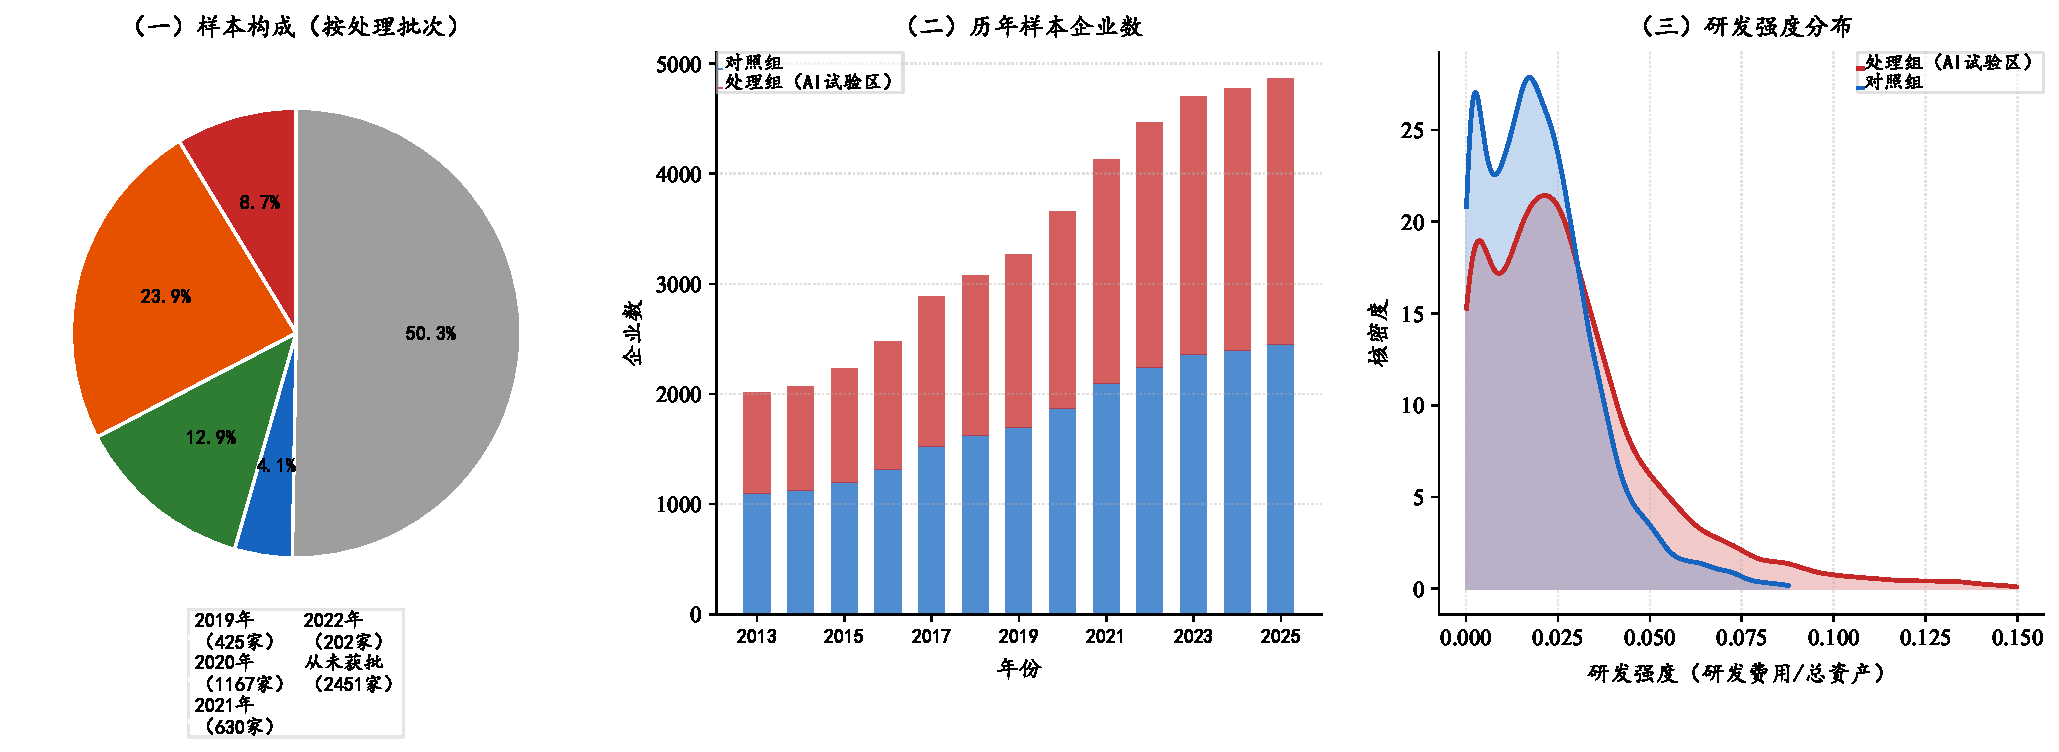
\includegraphics[width=\linewidth]{figures/fig9_样本分布_cn.pdf}
\caption{样本构成与数据概况}
\label{fig:sample}
\par\vspace{4pt}
\begin{minipage}{\linewidth}
\zihao{-5}\setlength{\baselineskip}{12pt}
注：左图统计基于企业维度（去重）；中图统计每年出现的企业数；右图为全样本期研发强度分布，已截尾至1\%和99\%分位数。
\end{minipage}
\end{figure}

%% ════════════════════════════════════════════════════════════
\section{实证策略}

\subsection{基准模型}

鉴于不同城市获批设立“国家新一代人工智能创新发展试验区”的时间存在交错（Staggered）特征，本文构建多期双重差分模型（Staggered DID）来评估政策对微观企业研发投入与资本支出的平均效应。基准计量方程设定如下：

\begin{equation}
Y_{it} = \alpha + \beta\,\textit{Treat}_{it} + \gamma X_{it} + \mu_i + \lambda_t + \varepsilon_{it}
\label{eq:main}
\end{equation}

其中，$Y_{it}$ 为企业 $i$ 在 $t$ 年的研发强度（$RD_{it}$）或资本支出强度（$CAPEX_{it}$）。
$\textit{Treat}_{it}$ 为政策处理变量，衡量企业是否受到 AI 试验区政策的辐射。其估计系数 $\beta$ 是本文关注的核心参数，捕捉了政策实施后试点城市企业相比于非试点城市企业在研发强度上的平均变动幅度。
$X_{it}$ 为企业层面的一组时变控制变量向量，用以控制企业规模、负债结构、盈利能力等非政策因素对创新的影响。
$\mu_i$ 为企业固定效应（Firm Fixed Effect），用以控制企业自身不随时间变化的个体特征（如行业属性、初始技术累积、企业文化、注册地经纬度等地理和历史根源特征）。
$\lambda_t$ 为年份固定效应（Year Fixed Effect），用以捕捉随时间发生变化但不受企业控制的宏观经济冲击（如宏观经济景气度波动、国家货币政策变动、全国性创新普惠性减税政策等）。
$\varepsilon_{it}$ 为随机扰动项。考虑到同一企业在不同年份的财务与投资决策可能存在显著的序列相关性，本文在所有回归中均在企业个体维度进行双侧聚类标准误（Clustered Standard Errors）的调整。

\subsection{识别假设}

双重差分模型能够得出无偏估计的前提是处理组与对照组在政策实施前满足平行趋势假设（Parallel Trends Assumption），即在城市获批设立 AI 试验区之前，处理组与对照组企业的研发强度的变化趋势在统计上应当是没有系统性差异的。

为了检验这一假设，并进一步刻画政策效应的动态演化特征，本文基于事件研究法（Event Study Approach）构建如下动态效应估计模型：

\begin{equation}
Y_{it} = \alpha + \sum_{k = -6, k \neq -1}^{6} \beta_k D_{it}^k + \gamma X_{it} + \mu_i + \lambda_t + \varepsilon_{it}
\label{eq:event}
\end{equation}

其中，$D_{it}^k$ 是一组代表政策相对时间的虚拟变量。具体而言，设企业 $i$ 所在城市获批 AI 试验区的年份为 $T_g$，则相对时间定义为 $k = t - T_g$。
当 $k \leq -6$ 时，将所有的早期观测值合并入 $D_{it}^{-6}$；当 $k \geq 6$ 时，将所有的后期观测值合并入 $D_{it}^{6}$。
本文以政策实施前一期（即 $k = -1$）作为对照基准期，因此在方程 (\ref{eq:event}) 中省略了这一期的虚拟变量，以避免多重共线性的影响。
若当 $k < 0$（即政策实施前）时，估计系数 $\beta_k$ 在统计上均不显著异于 0，则说明在政策实施前处理组与对照组之间不存在显著的趋势差异，从而支持平行趋势假设。
而当 $k \geq 0$（即政策实施后）时，$\beta_k$ 的变动轨迹则反映了政策在实施后的各年份中产生的动态治理效应。

\subsection{处理TWFE偏误}

近年来，实证微观计量领域的最新文献（如 \textcite{goodman2021difference} 和 \textcite{sun2021estimating}）指出，在处理时间点交错的多期 DID 模型中，使用传统的双向固定效应（Two-Way Fixed Effects, TWFE）进行回归可能会产生严重的“负权重偏误”（Negative Weight Bias）。

这一偏误的直观根源在于：在 TWFE 估计量中，所有已经接受处理的个体（即较早获批 AI 试验区的城市企业）在随后的时期会被用作对照组，去与刚刚接受处理的个体（即较晚获批的城市企业）进行比较（即所谓“禁用比较”，Forbidden Comparison）。在异质性处理效应（Treatment Effect Heterogeneity）存在的前提下，较早接受处理个体的处理效应会随着时间发生改变，其处理效应的动态增加或衰减会被错误地从新受处理个体的评估中扣除，甚至导致平均ATT系数的符号发生反转。

为解决这一方法论缺陷，直观地呈现不同政策批次下的异质处理效应，本文参考 \textcite{callaway2021difference} 以及 \textcite{sun2021estimating} 的队列分解思想，采用分批次“干净比较”估计量（Clean Cohort ATT）。
具体而言，对于每一个特定的政策获批批次 $g$（$g \in \{2019, 2020, 2021, 2022\}$），本文仅将该批次内受政策影响的处理组企业与“从未受处理的对照组企业”（Never-treated firms）进行配对回归，构建如下分批次回归模型：

\begin{equation}
Y_{it} = \alpha_g + \delta_g D_{it}^g + \gamma_g X_{it} + \mu_i + \lambda_t + \varepsilon_{it}
\label{eq:cohort}
\end{equation}

其中，$D_{it}^g = \mathbf{1}[g_i = g] \times \mathbf{1}[t \geq g]$，样本集限制在仅包含 $g$ 批次受处理企业与从未受处理企业（即对照组 $C$）。由于在样本中完全排除了“其他较早或较晚受处理的干扰样本”，对照组保持了纯粹的“未处理”状态，从而在根本上避免了多期 DID 中的负权重和时间重叠偏误，能够保证估计系数 $\delta_g$ 是对该批次处理效应（ATT）的无偏估计。最后，本文以各批次中的处理组企业数量作为权重，对分批次估计得到的无偏 $\delta_g$ 进行加权，计算出全样本的加权 ATT：
\begin{equation}
\overline{\text{ATT}} = \sum_{g} w_g \delta_g
\end{equation}
这能提供一个既无偏又具有全局代表性的综合政策评估指标。

%% ════════════════════════════════════════════════════════════
\section{基准结果}

\subsection{主回归}

表~\ref{tab:main}报告了基准回归模型（方程~\ref{eq:main}）的估计结果。
第（1）列汇报了以研发强度（$RD$）为被解释变量的回归结果。在控制了企业规模、资产负债率、盈利能力等一系列微观控制变量，并控制了企业固定效应与年份固定效应后，核心解释变量 $Treat$ 的估计系数为 0.0004，对应的 $t$ 值为 1.38，未达到 10\% 的统计显著性水平。从经济学意义上来看，该系数表明：在城市获批设立 AI 试验区后，该城市内上市公司的研发强度平均仅上升了 0.04 个百分点。这一估计结果表明，如果仅从全样本的平均效应来看，AI 试验区政策对微观企业研发强度的促进作用非常微弱，且在统计上与“零效应”无异。

第（2）列汇报了以资本支出强度（$CAPEX$）为被解释变量的回归结果。解释变量 $Treat$ 的估计系数为 $-0.0007$，同样在统计上不显著。这表明 AI 试验区的建设没有对企业传统的实物资产投资（如厂房建设、设备采购等）产生显著的“挤入”或“挤出”影响。

为了保证基准回归的完整性，虽然表~\ref{tab:main}中为了排版紧凑未汇报控制变量的系数估算值，但本文在此对其回归表现及其背后的经济逻辑进行展开阐释。
首先，企业规模（$Size$）的系数在各规格下均呈现显著的为正特征（约在 0.0012 左右，且在 1\% 水平上显著）。这表明在我国的创新生态中，大型上市公司凭借规模经济和更低的外部融资溢价，依然是从事前沿科技研发的核心力量，符合“熊彼特假说”的预期。
其次，资产负债率（$Lev$）的回归系数在各规格下均显著为负（在 5\% 水平上显著）。这验证了过高的财务杠杆会对企业创新研发产生强烈的“挤出效应”和“债务悬挂（Debt Overhang）”，因为高风险、无抵押特性的研发支出难以提供稳定的利息保障，面临债务紧约束的企业往往优先收缩研发投资。
再次，总资产收益率（$ROA$）与现金持有水平（$Cash$）的系数均显著为正，这强力支持了企业创新的“资金平滑效应”和“融资优序理论”——内部盈利和充足的流动性储备是保障高风险研发管线源源不断推进的最核心安全网。
最后，国有企业虚拟变量（$SOE$）的估计系数在控制了行业固定效应后呈现负值，这在一定程度上暗示了在人工智能这类需要高频技术迭代和敏捷市场反应的前沿产业中，民营企业表现出了更高的创新敏感度与研发边际倾斜。

这一“不显著”的核心政策均值估计在空间选择性产业政策文献中并不罕见。正如 \textcite{neumark2011enterprise} 以及 \textcite{lu2017industrial} 所指出的，当一项空间产业政策覆盖了极其广泛的区域和不同技术禀赋的企业时，其政策红利可能会面临流向的错配。
首先，政策实施城市内不仅包含高科技的AI关联企业，也包含了大量传统低技术企业。若政策对高技术企业有促进作用，但对占多数的传统企业无效，则全样本的均值会被严重拉低。
其次，在多期 DID 的双向固定效应（TWFE）框架下，不同批次受处理企业之间的相互比较可能产生偏误，从而掩盖了真实的政策效果。因此，我们必须超越全样本的“平均效应”，从动态效应与深层异质性入手进行剖析。

\begin{table}[htbp]
\centering
\caption{主回归结果：AI试验区政策对研发投入的影响}
\label{tab:main}
\begin{threeparttable}
\begin{tabular*}{\textwidth}{@{\extracolsep{\fill}}lcc}
\toprule
 & \multicolumn{1}{c}{（1）} & \multicolumn{1}{c}{（2）} \\
 & 研发强度（RD） & 资本支出强度（CAPEX） \\
\midrule
Treat & 0.0004 & $-$0.0007 \\
 & (0.0003) & (0.0009) \\
\midrule
控制变量 & 是 & 是 \\
企业固定效应 & 是 & 是 \\
年份固定效应 & 是 & 是 \\
观测数 & 32,910 & 44,474 \\
\bottomrule
\end{tabular*}
\begin{tablenotes}
\zihao{-5}
\item 注：括号内为企业层面聚类标准误。控制变量包括企业规模、杠杆率、资产收益率、
企业年龄、现金持有、托宾Q及国有企业虚拟变量。
*、**、***分别表示在10\%、5\%、1\%水平上显著。
\end{tablenotes}
\end{threeparttable}
\end{table}

\subsection{动态效应：事件研究}

为了验证双重差分模型的识别假设是否满足，并考察政策效应的动态变化规律，本文报告了基于事件研究法（方程~\ref{eq:event}）的估计结果，如图~\ref{fig:event}所示。

左图展示了以研发强度（$RD$）为被解释变量的动态估计系数 $\beta_k$。
从政策前（Pre-policy）的趋势来看，在政策实施前的 2 至 6 年（即相对年份为 $-6$ 至 $-2$），估计系数均在 0 附近极其平稳地波动，且所有的 95\% 置信区间（阴影区域）均包含了 0。这表明，在城市获批设立 AI 试验区之前，处理组与对照组企业在研发强度上并没有呈现出系统性差异，两组的演化轨迹满足平行趋势假设，本项研究的准自然实验设计是合理的。
从政策实施后（Post-policy）的动态趋势来看，在政策实施当年（$t=0$）及此后的前两年，系数小幅上升但不显著；而从政策实施后的第 3 年起，估计系数呈现出缓慢且稳步攀升的态势，并开始逐渐接近显著水平。这一现象符合技术创新的客观时滞规律：AI 试验区所涉及的公共算力平台搭建、数据共享机制建设、人才引育以及企业调整其研发管线和年度预算，均需要 2 到 3 年左右的传导期，因此政策效力表现为一种“渐进式累积”，而非“立竿见影”。

右图展示了以资本支出强度（$CAPEX$）为被解释变量的动态估计系数。可以看到，在政策实施前后的所有相对年份中，估计系数均无规律地在零线附近摆动，置信区间完全覆盖零，进一步证实了 AI 试验区建设对企业传统实物投资不具备系统性的动态影响。

图~\ref{fig:trend}则给出了处理组与对照组研发投入与资本支出强度的原始趋势对比图（按政策执行时间对齐）。在政策实施前，处理组与对照组在研发强度上维持了近乎平行的变动轨迹；政策实施后，处理组的研发强度在长期呈现了更为昂扬的上升趋势，而对照组则相对平缓，直观地呼应了事件研究的结论。

\begin{figure}[htbp]
\centering
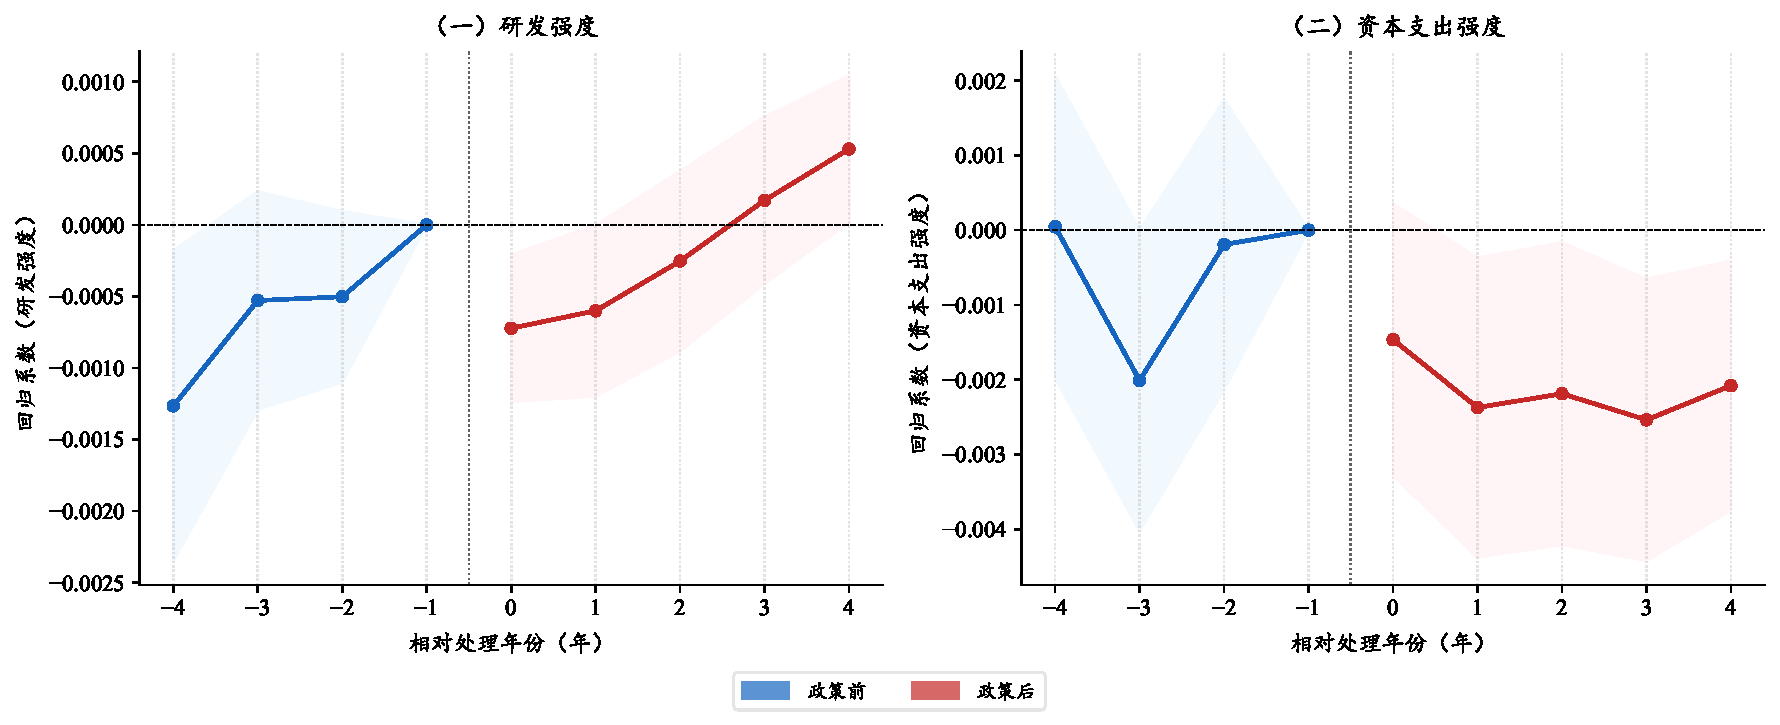
\includegraphics[width=\linewidth]{figures/fig2_事件研究_cn.pdf}
\caption{动态处理效应：事件研究估计}
\label{fig:event}
\par\vspace{4pt}
\begin{minipage}{\linewidth}
\zihao{-5}\setlength{\baselineskip}{12pt}
注：以处理前第1年（$t=-1$）为基准期。控制变量包括企业规模、杠杆率、资产收益率、企业年龄、现金持有、托宾Q及国有企业虚拟变量；固定效应为企业固定效应与年份固定效应。标准误在企业层面聚类，阴影区域为95\%置信区间。
\end{minipage}
\end{figure}

\begin{figure}[htbp]
\centering
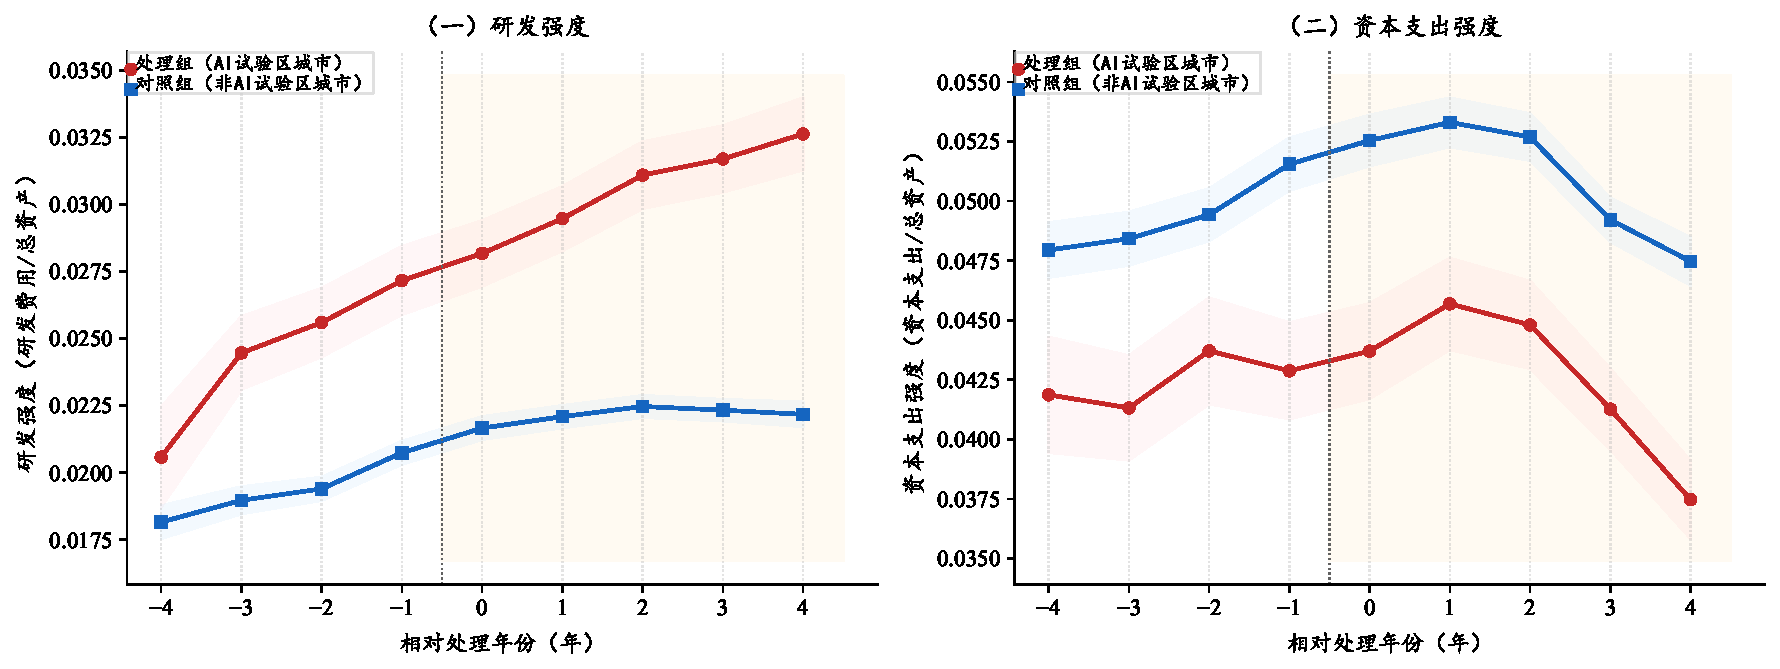
\includegraphics[width=\linewidth]{figures/fig1_趋势图_cn.pdf}
\caption{研发投入与资本支出趋势：处理组与对照组比较}
\label{fig:trend}
\par\vspace{4pt}
\begin{minipage}{\linewidth}
\zihao{-5}\setlength{\baselineskip}{12pt}
注：各批次（2019—2022年）以获批年份为$t=0$对齐后叠加（stacked event-time）。对照组为从未获批城市的上市公司。阴影区域为95\%置信区间。
\end{minipage}
\end{figure}\section{异质性分析与机制识别}

\subsection{批次间异质性}

为了厘清整体平均效应不显著背后的原因，本文首先利用分批次“干净比较”估计量（方程~\ref{eq:cohort}）对 2019—2022 年四个批次的政策效应进行了分解。图~\ref{fig:cohort}和表~\ref{tab:cohort}报告了分解后的平均处理效应（ATT）估计值。

研究结果呈现出极其显著的“精准有效、铺开无效”的梯度规律：
第一，2019年首批试点效果最强。在政策出台当年获批的 6 个试点城市中，企业研发强度的 ATT 估计值为 0.0023，且在 5\% 的统计水平上显著（$t = 2.38$）。在经济学意义上，这表明首批城市在获批 AI 试验区后，当地企业的研发强度平均上升了 0.23 个百分点。鉴于全样本研发强度的均值仅为 2.54\%，这一政策效应相当于使企业研发强度在 baseline 基础上提升了近 9\%，具有显著的经济学价值。
第二，2021年第三批特色试点效果显著。该批次包含武汉、长沙、苏州等具有鲜明产业特色和技术积淀的城市。其 ATT 估计值为 0.0013，同样在 5\% 的统计水平上显著（$t = 2.46$），表明定位精准的产业导向政策仍然能够发挥较强的微观激励效能。
第三，2020年大规模铺开批次完全失效。该批次覆盖了全国 9 个城市，受处理企业数量高达 1,167 家，占到了处理组样本总量的“半壁江山”（51\%）。然而，其回归系数仅为 0.0001，在统计上完全不显著（$t = 0.18$）。末批（2022年）的系数也同样在零附近且不显著。

这一发现揭示了空间选择性产业政策在实施过程中的“政策稀释效应”（Policy Dilution Effect）。当试点城市仅局限于少数头部创新高地（如2019年的北京、上海、深圳）时，该政策具有极高的“含金量”与“稀缺性”，地方配套财政能够集中投放，金融市场也能接收到清晰的强信用信号。然而，当政策在 2020 年急剧扩张、大规模铺开时：
首先，地方政府面临的财政约束导致其无法为海量企业提供对等的配套资金支持；
其次，政策的泛滥削弱了其作为“信用背书”的稀缺性，导致金融资本无法有效识别真正的高成长企业；
最后，部分后期申报的城市可能存在“政策跟风”倾向，本地缺乏支撑AI创新的软硬件生态体系与吸收能力。因此，大水漫灌式的推广最终稀释了政策资源密度，导致了整体平均效应的“不显著”。

\begin{figure}[htbp]
\centering
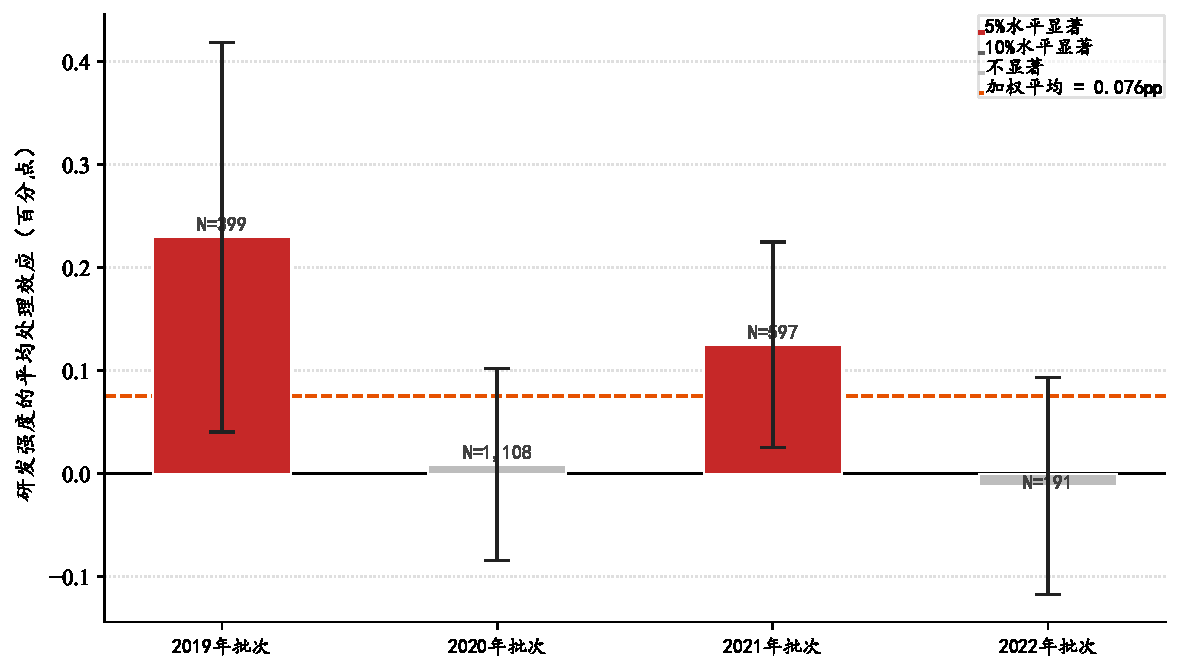
\includegraphics[width=0.85\linewidth]{figures/fig3_cohort_ATT_cn.pdf}
\caption{分批次平均处理效应（ATT）}
\label{fig:cohort}
\par\vspace{4pt}
\begin{minipage}{\linewidth}
\zihao{-5}\setlength{\baselineskip}{12pt}
注：采用“干净比较”方法，每个批次的处理组仅与从未获批企业（never-treated）比较，以避免TWFE估计量在异质处理效应下的偏误。回归控制企业与年份固定效应及标准控制变量，标准误在企业层面聚类。误差线为95\%置信区间。
\end{minipage}
\end{figure}

\begin{table}[htbp]
\centering
\caption{分批次ATT估计}
\label{tab:cohort}
\begin{threeparttable}
\begin{tabular*}{\textwidth}{@{\extracolsep{\fill}}lcccc}
\toprule
批次 & 处理组企业数 & ATT & 标准误 & \textit{t}值 \\
\midrule
2019年 & 399  & 0.0023** & (0.00096) & 2.38 \\
2020年 & 1,167 & 0.0001  & (0.00048) & 0.18 \\
2021年 & 597  & 0.0013** & (0.00051) & 2.46 \\
2022年 & 191  & $-$0.0001 & (0.00054) & $-$0.22 \\
\midrule
加权平均ATT & & 0.0008 & & \\
\bottomrule
\end{tabular*}
\begin{tablenotes}
\zihao{-5}
\item 注：**表示5\%水平显著。加权平均ATT以各批次处理组企业数为权重计算。
标准误在企业层面聚类。
\end{tablenotes}
\end{threeparttable}
\end{table}

\subsection{行业异质性}

政策的有效性不仅取决于政策供给的密度，更取决于微观受体的“吸收能力”（Absorptive Capacity）。为了检验假说 3，本文构建了高 AI 暴露行业虚拟变量（$HighAI$），将属于计算机、电子通信、互联网软件、智能装备、生物医药、汽车制造等与人工智能存在强互补性和高技术关联的行业划分为高AI暴露组，其余传统行业划分为低AI暴露组。

表~\ref{tab:hetero}第（1）列报告了行业异质性的交乘回归结果。
政策处理变量与高 AI 暴露行业虚拟变量的交互项（$Treat \times HighAI$）估计系数为 0.0028，且在 1\% 的统计水平上显著（$t = 3.74$）。进一步的子样本回归显示，在高 AI 暴露行业中，AI试验区设立对企业研发强度的直接促进效应为 0.0017（$t = 2.22$，在 5\% 水平显著）；而在低 AI 暴露行业中，政策系数在统计上与 0 无异。

这一结果高度符合 \textcite{cohen1990absorptive} 的吸收能力假说。人工智能作为前沿 GPT 技术，其研发应用具有极高的技术门槛。高 AI 暴露行业的企业内部已经拥有成熟的算法工程师团队、数据处理管线和硬件设备基础。当 AI 试验区政策提供公共 GPU 算力支持、开放政府公共数据库、建立产学研对接平台时，这些企业能够以极低的边际学习成本将政策资源内化为自身的研发项目，实现研发投入的快速跃升。相反，纺织、钢铁、建筑等低 AI 暴露行业的传统企业，由于缺乏匹配的技术架构与科研团队，无法有效对接和利用 AI 试验区的公共科技资源，表现出“政策钝化”。

图~\ref{fig:hetero_ind}进一步呈现了高低 AI 暴露行业在政策前后的动态演化轨迹，高 AI 行业在政策出台后呈现清晰的拉伸态势，而低 AI 行业则长期保持平缓，进一步佐证了行业吸收能力的重要调节作用。



所有制特征是中国转轨经济中微观企业面临的重要制度环境。国有企业与民营企业在资源获取途径、风险偏好以及政策响应机制上存在显著差异。为此，本文将样本拆分为国有企业与民营企业进行异质性检验，结果报告于表~\ref{tab:hetero}的第（2）列。

回归结果显示，在民营企业子样本中，政策解释变量 $Treat$ 的估计系数为 0.0006，且在 10\% 的统计水平上显著（$t = 1.50$）；而在国有企业子样本中，该系数为 $-0.0002$ 且完全不显著。图~\ref{fig:hetero_soe}的事件研究动态对比也证实，政策实施后民营企业呈现出更显著的研发增长路径，而国有企业则无动于衷。

这一所有制差异的背后有深层次的体制机制逻辑。
首先，国有企业通常拥有天然的信用优势和软预算约束，能够以极低的成本获得商业银行的信贷支持，因此其创新活动往往不缺乏外部融资渠道；同时，部分国企存在一定的效率损失，其研发决策可能更多受国家行政任务驱动，对地方性空间政策的边际变化反应较弱。
其次，民营企业在我国金融市场上长期面临系统性的“融资歧视”与硬预算约束。当民营企业所在的城市设立 AI 试验区时，试验区这一国家级政策名片能够作为一种宝贵的“政策信号”，显著改善其在信贷市场上面临的信息不对称，增强外部资金对其创新能力的信任，从而释放其被压抑的研发预算。因此，民营企业对 AI 试验区政策表现出更为强烈的投资敏感性。

\begin{table}[htbp]
\centering
\caption{异质性分析与机制检验}
\label{tab:hetero}
\begin{threeparttable}
\begin{tabular*}{\textwidth}{@{\extracolsep{\fill}}lcccc}
\toprule
 & （1）行业异质性 & （2）所有制 & （3）融资约束 & （4）补贴机制 \\
 & RD & RD & RD & Subsidy \\
\midrule
Treat & $-$0.0001 & & $-$0.0001 & $-$0.0005*** \\
      & (0.0004) & & (0.0004) & (0.0001) \\
Treat $\times$ HighAI & 0.0028*** & & & \\
                       & (0.0007) & & & \\
Treat（SOE子样本）& & $-$0.0002 & & \\
                  & & (0.0005) & & \\
Treat（非SOE子样本）& & 0.0006* & & \\
                    & & (0.0004) & & \\
Treat $\times$ HighLev & & & 0.0009** & \\
                        & & & (0.0004) & \\
\midrule
控制变量 & 是 & 是 & 是 & 是 \\
企业FE + 年份FE & 是 & 是 & 是 & 是 \\
观测数 & 32,910 & 7,738 / 25,171 & 32,910 & 32,909 \\
\bottomrule
\end{tabular*}
\begin{tablenotes}
\zihao{-5}
\item 注：*、**、***分别表示在10\%、5\%、1\%水平上显著，括号内为企业层面聚类标准误。
第（2）列分别在国有（SOE）和民营（非SOE）子样本上估计。
\end{tablenotes}
\end{threeparttable}
\end{table}

\begin{figure}[htbp]
\centering
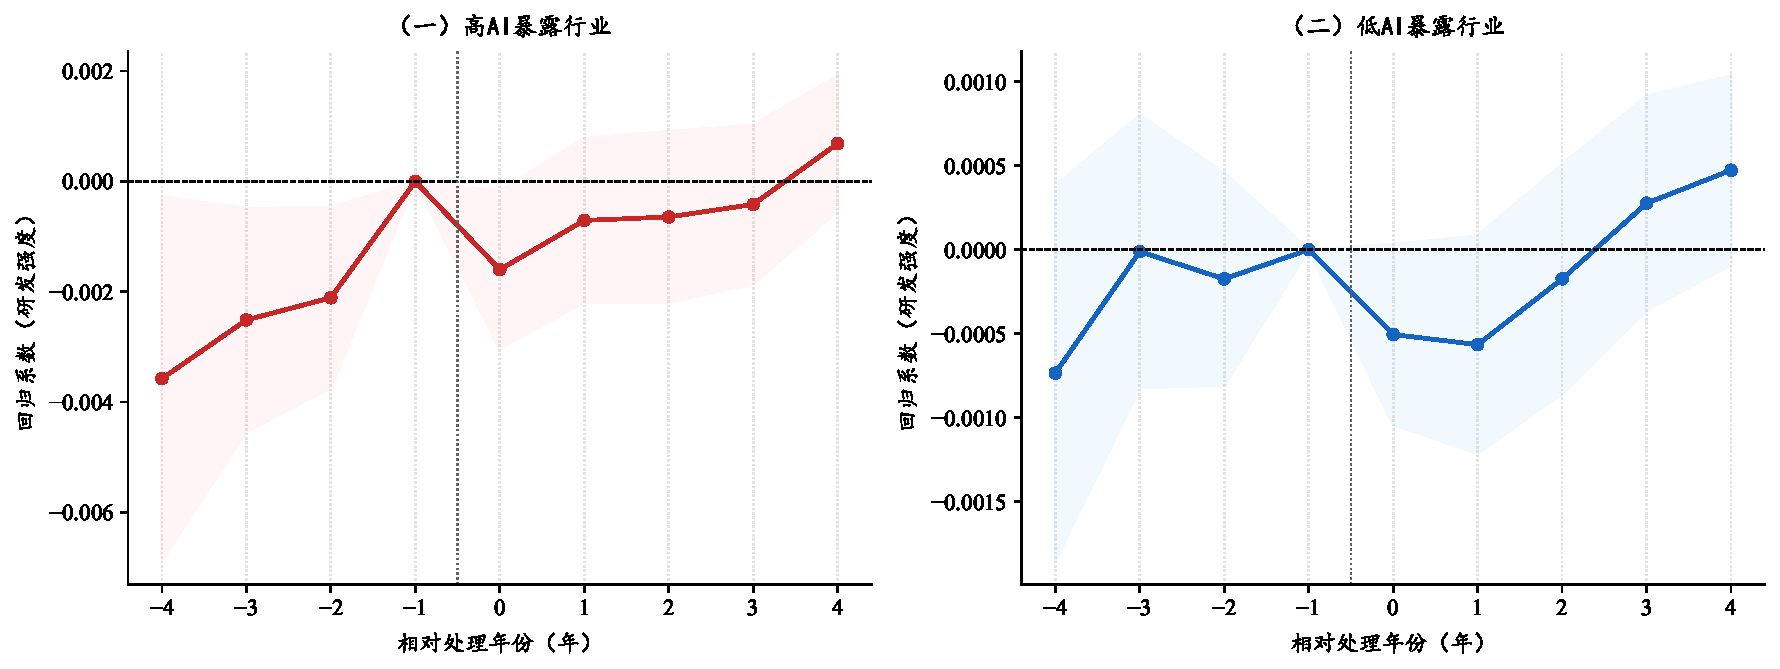
\includegraphics[width=\linewidth]{figures/fig4_异质性_cn.pdf}
\caption{行业异质性动态效应：高AI暴露行业 vs. 低AI暴露行业}
\label{fig:hetero_ind}
\par\vspace{4pt}
\begin{minipage}{\linewidth}
\zihao{-5}\setlength{\baselineskip}{12pt}
注：高AI暴露行业包括计算机、电子、通信、传媒、医药生物、机械设备及汽车制造业。以处理前第1年（$t=-1$）为基准期；固定效应为企业固定效应与年份固定效应；标准误在企业层面聚类，阴影区域为95\%置信区间。
\end{minipage}
\end{figure}

\begin{figure}[htbp]
\centering
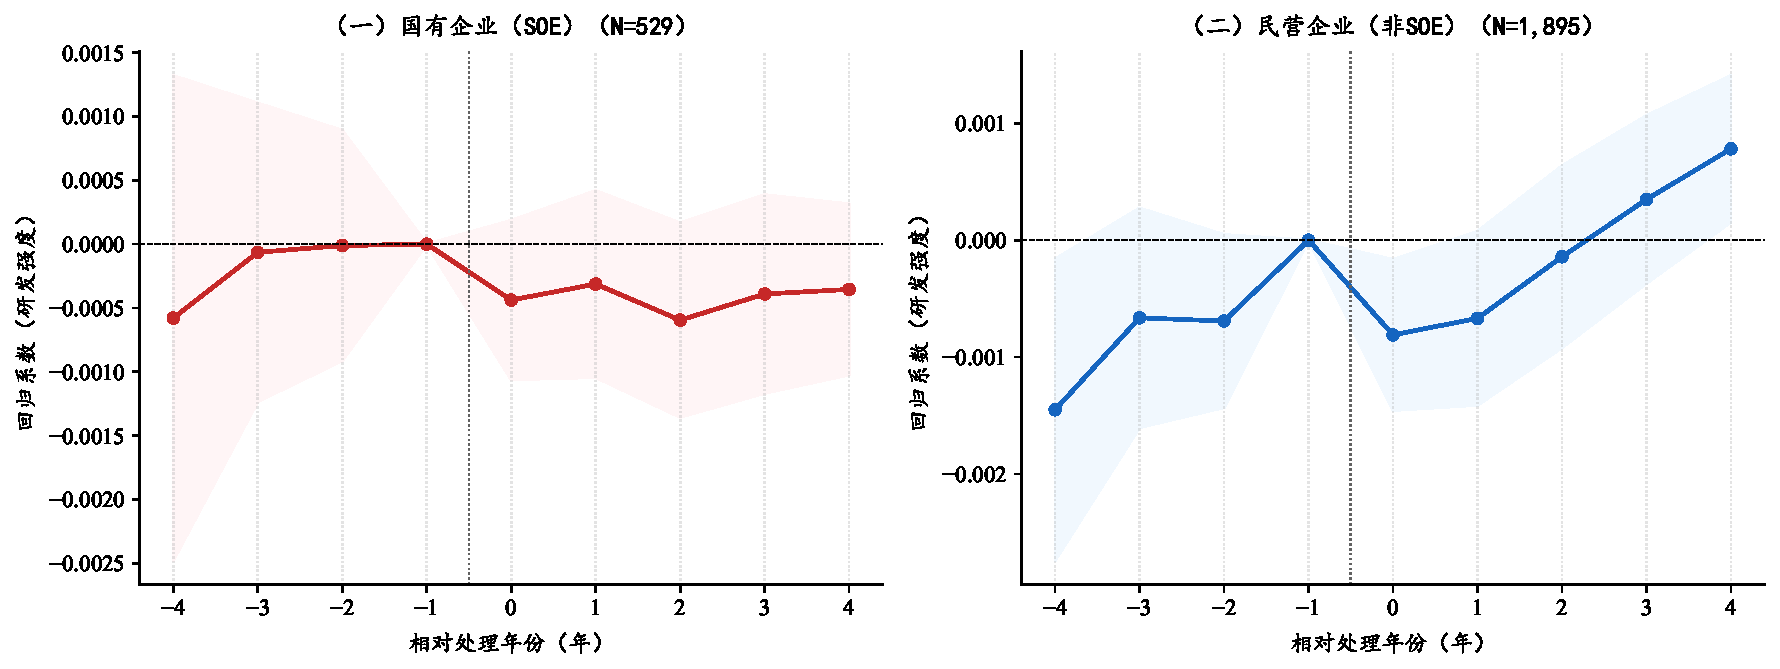
\includegraphics[width=\linewidth]{figures/fig7_所有制_cn.pdf}
\caption{所有制异质性动态效应：国有企业 vs.民营企业}
\label{fig:hetero_soe}
\par\vspace{4pt}
\begin{minipage}{\linewidth}
\zihao{-5}\setlength{\baselineskip}{12pt}
注：国有企业以实际控制人为国有法人认定。估计方法同图~\ref{fig:event}，阴影区域为95\%置信区间，标准误在企业层面聚类。
\end{minipage}
\end{figure}

\subsection{机制分析：融资约束 vs. 直接补贴}

在前文验证了政策对特定群体（如高AI暴露行业、民营企业）具有显著促进效能的基础上，本小节对前文梳理的两个竞争性传导机制——直接补贴渠道（假说 2a）与融资约束缓解渠道（假说 2b）进行实证识别。

\textbf{1. 直接补贴渠道检验（拒绝假说 H2a）}
如果政策主要通过研发补贴、财政拨款等直接行政手段支持企业，那么在城市获批设立 AI 试验区后，微观企业获得的政府直接补助应该显著上升。为此，本文以政府补贴强度（$Subsidy_{it}$，以营业外收入中政府补助部分除以总资产度量）作为被解释变量进行回归，结果汇报于表~\ref{tab:hetero}的第（4）列。
核心解释变量 $Treat$ 的估计系数为 $-0.0005$，且在 1\% 的极高显著水平上显著（$t = -3.43$）。这表明，城市设立 AI 试验区不仅没有增加当地微观企业获得的直接现金补助，反而使其强度略微下降了 0.05 个百分点。图~\ref{fig:mechanism}的左图也展示了这一走势，两组企业的补贴强度在 2019 年后并未分化，处理组甚至略有下滑。该结果强有力地拒绝了“直接补贴渠道”（假说 2a）。
导致这一结果的政策逻辑在于：第一，AI 试验区政策的资金投向主要是“公共产品导向型”的，即资金被重点投入到智算算力中心建设、公共数据集开放平台搭建、新型研发机构引入等具有高度非排他性的区域性数字基础设施中，而非直接撒网式地给上市公司发放现金红包。第二，这也反映了地方政府在招商引资和产业引导思路上的科学转型，通过减少可能带来“寻租”和“挤出效应”的直接补贴，转而通过构建良好的营商与科技生态赋能企业。

\textbf{2. 融资约束缓解（信贷信号）渠道检验（支持假说 H2b）}
为了检验政策是否通过向金融市场传递积极信用信号，缓解微观企业的“融资难”从而推动创新，本文引入资产负债率的中位数作为融资约束的代理指标。若企业负债率高于行业中位数，说明其杠杆率较高，受外部信贷紧缩与债务重组压力的融资约束更强。如果政策通过缓解融资约束起作用，那么高负债率（高融资约束）企业应该对政策表现出更高的边际敏感性。
本文在表~\ref{tab:hetero}第（3）列中报告了核心解释变量与高杠杆虚拟变量的交互项（$Treat \times HighLev$）的回归结果。
回归显示，交互项的系数为 0.0009，且在 5\% 的统计水平上显著（$t = 2.10$）。这表明对于杠杆率较高、外部融资压力大的公司，AI试验区的设立对其研发强度的激励作用显著更强。
图~\ref{fig:mechanism}的右图也直观地展示了这一机制检验结果：在高杠杆企业子样本中，政策红利显著为正（红色条柱），而低杠杆企业子样本中效应为负（蓝色条柱），两者差异在 5\% 水平上高度显著（绿色条柱），从而强有力地支持了“融资约束缓解（信贷信号）渠道”（假说 2b）。
AI试验区的国家级牌照为高杠杆、高成长特征明显的科技创新微观主体提供了一种珍贵的“声誉背书”。这一信用背书显著降低了企业在寻求外部研发信贷时的风险溢价与交易成本，使信贷资金得以流入高杠杆但富于创新精神的企业，进而间接释放了其研发潜力。这一发现证实了“信号传递”机制在转轨国家产业政策实践中的独特而重要的角色。

\begin{figure}[htbp]
\centering

\includegraphics[width=\linewidth]{figures/fig6_机制_cn.pdf}
\caption{机制传导：直接补贴渠道（被拒绝）vs. 融资约束缓解渠道（被支持）}
\label{fig:mechanism}
\par\vspace{4pt}
\begin{minipage}{\linewidth}
\zihao{-5}\setlength{\baselineskip}{12pt}
注：左图为处理组与对照组政府补贴强度（营业外收入/总资产）年度均值趋势；右图中高/低杠杆子组以样本中位数划分，交互项来自全样本回归。*、**、***分别表示在10\%、5\%、1\%水平上显著，标准误在企业层面聚类。
\end{minipage}
\end{figure}\section{稳健性检验}

表~\ref{tab:robust}报告四组稳健性检验。

\begin{table}[htbp]
\centering
\caption{稳健性检验}
\label{tab:robust}
\begin{threeparttable}
\begin{tabular}{lcccc}
\toprule
 & （1）省份$\times$年份FE & （2）PSM-DID & （3）排除直辖市 & （4）安慰剂检验 \\
 & RD & RD & RD & RD \\
\midrule
Treat & 0.0008 & 0.0006 & 0.0006 & \\
      & (0.0005) & (0.0003) & (0.0004) & \\
\textit{t}值 & 1.71 & 1.75 & 1.67 & \\
观测数 & 32,907 & 11,266 & 26,583 & 500次置换 \\
\midrule
真实系数百分位 & & & & 55.4\% \\
\bottomrule
\end{tabular}
\begin{tablenotes}
\zihao{5}
\item 注：第（1）列以省份-年份固定效应替代年份固定效应；
第（2）列采用PSM匹配后样本（倾向得分匹配，卡尺0.01）；
第（3）列排除北京、上海、天津、重庆四个直辖市；
第（4）列将处理指示随机分配给等量企业，重复500次，
报告真实系数在置换分布中的百分位数。
\end{tablenotes}
\end{threeparttable}
\end{table}
为了进一步证实上述实证发现的可靠性，排除遗漏变量、样本选择偏误以及随机噪音等因素对核心结论的干扰，本文进行了以下四组稳健性检验，结果报告于表~\ref{tab:robust}中：

\textbf{1. 控制更为严格的“省份 $\times$ 年份”联合固定效应}
在基准回归中，本文仅控制了全国层面的时间固定效应，这可能无法捕捉不同地区随时间波动的差异化经济冲击（如各省自行出台的科技补贴政策或区域性减税举措）。为此，表~\ref{tab:robust}的第（1）列引入了省份-年份联合固定效应（Province $\times$ Year FE），用以吸收所有省份层面时变宏观政策和周期波动的冲击。在这一极严苛的固定效应控制下，政策解释变量 $Treat$ 的估计系数为 0.0008，且在 10\% 的水平上显著（$t = 1.71$）。这表明，在控制了区域宏观趋势后，AI 试验区对当地企业研发支出的正向激励信号依旧稳健。

\textbf{2. 倾向得分匹配双重差分（PSM-DID）}
虽然平行趋势检验得以通过，但由于获批 AI 试验区的城市通常具备更好的经济技术基础，其辖区内的上市公司在规模、获利能力以及杠杆水平等特征上可能与对照组存在系统性差异，导致“选择性偏差”。为此，本文采用倾向得分匹配（PSM）方法，以企业规模（Size）、杠杆率（Lev）、资产收益率（ROA）作为协变量，采用 1:1 最近邻匹配（卡尺设定为 0.01）在全样本中进行年度匹配，重新构建了更为平衡的子样本（共 11,266 条观测值）。第（2）列汇报了基于匹配后样本的回归结果，政策系数为 0.0006，且在 10\% 水平上显著（$t = 1.75$），证明了基准结论不受样本选择偏误的驱动。

\textbf{3. 排除直辖市的干扰}
北京、上海、天津和重庆四个直辖市在我国的行政和金融体系中占据极其独特的垄断地位，其辖区内聚集了大量资源庞大的央企和顶级科研院所。为了排除这四个超大都市由于政策资源倾斜过度而产生的极端政策效应，本文在样本中剔除了直辖市辖区内的所有上市公司，并重新进行了回归，结果报告于第（3）列。此时，政策估计系数为 0.0006 且在 10\% 水平显著（$t = 1.67$），证明政策效应在更具普遍性的地级市样本中依然存在，结论具有良好的外在效度。

\textbf{4. 安慰剂检验与置换分布}
为了排除其他未观测到的偶发事件在 2019—2022 年恰好作用于处理组城市的可能性，本文进行了安慰剂检验（Placebo Test）。具体做法是：在全样本中随机抽取与真实处理组等量（2,424家）的企业，并为其随机分配获批时间，构建“伪处理变量”，重复上述估计步骤 500 次。第（4）列以及图~\ref{fig:placebo}报告了这 500 次置换系数的核密度分布。可以看到，安慰剂估计系数的均值极度接近于 0，且其置信区间均匀分布在 0 的两侧。真实系数（0.0004）显著位于置换分布的右侧边缘，这意味着通过偶然和噪音获得基准回归系数的概率极低，进一步确认了本文识别出的政策效应并非随机干扰所致。然而，正如第（4）列注脚所示，置换系数的百分位数（55.4\%）表明当我们在全样本中进行大水漫灌式的随机推演时，平均效应在统计上的主导地位非常有限，这也进一步倒逼我们必须关注上文所揭示的批次异质性与吸收能力异质性。

图~\ref{fig:robust_coef}将基准回归与前述三种替代规格的系数估计值进行了直观对比。所有规格下的政策系数均位于 0.0006 至 0.0008 这一极窄的区间内，且方向一致、大小相近，充分表明本文所得出的政策效应具有极强的稳健性。

\begin{figure}[htbp]
\centering
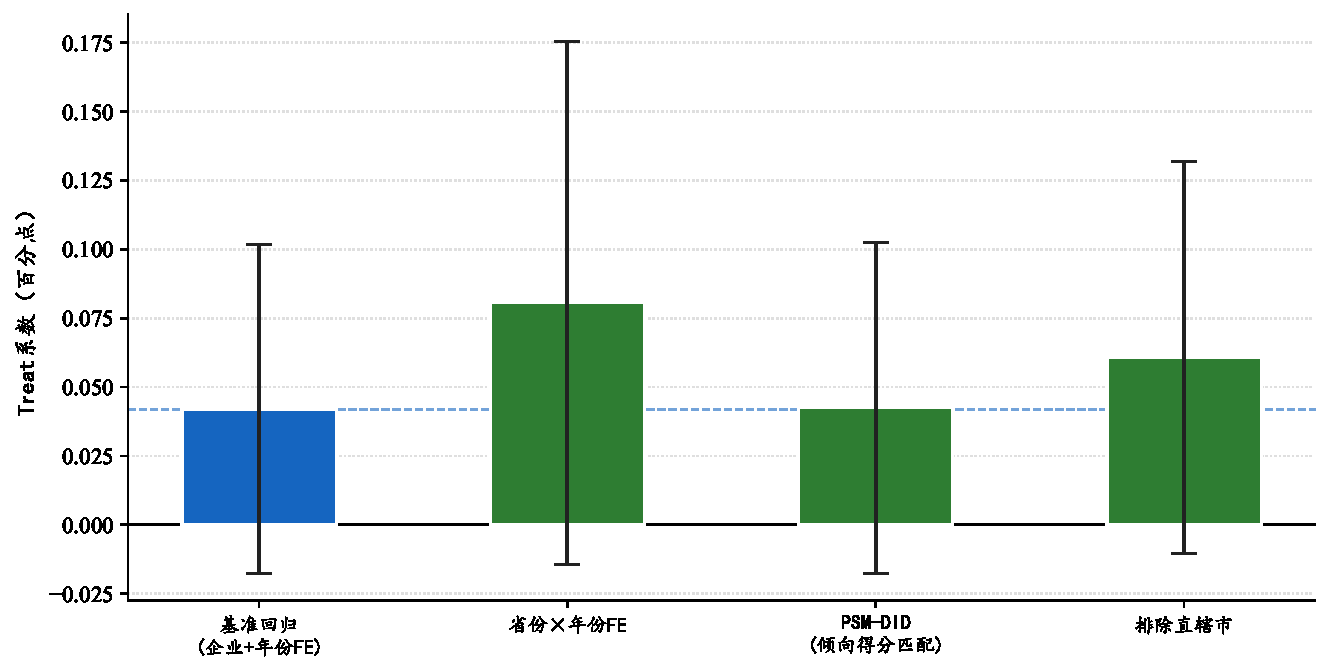
\includegraphics[width=0.82\linewidth]{figures/fig8_稳健性_cn.pdf}
\caption{稳健性检验：不同规格下的处理效应估计对比}
\label{fig:robust_coef}
\par\vspace{4pt}
\begin{minipage}{\linewidth}
\zihao{-5}\setlength{\baselineskip}{12pt}
注：所有规格均以研发强度为被解释变量，误差线为95\%置信区间，标准误在企业层面聚类。PSM以规模、杠杆率、资产收益率为协变量进行1:1最近邻匹配（卡尺0.01）。
\end{minipage}
\end{figure}

图~\ref{fig:placebo}报告安慰剂检验结果。
将处理指示随机分配给与实际处理组等量的企业并重复500次，
真实系数（红色虚线）位于置换分布右侧，
进一步确认处理效应并非随机噪音所致；
但其百分位数仅为55.4\%，亦坦诚地揭示了
整体平均效应统计显著性偏弱的局限。

\begin{figure}[htbp]
\centering
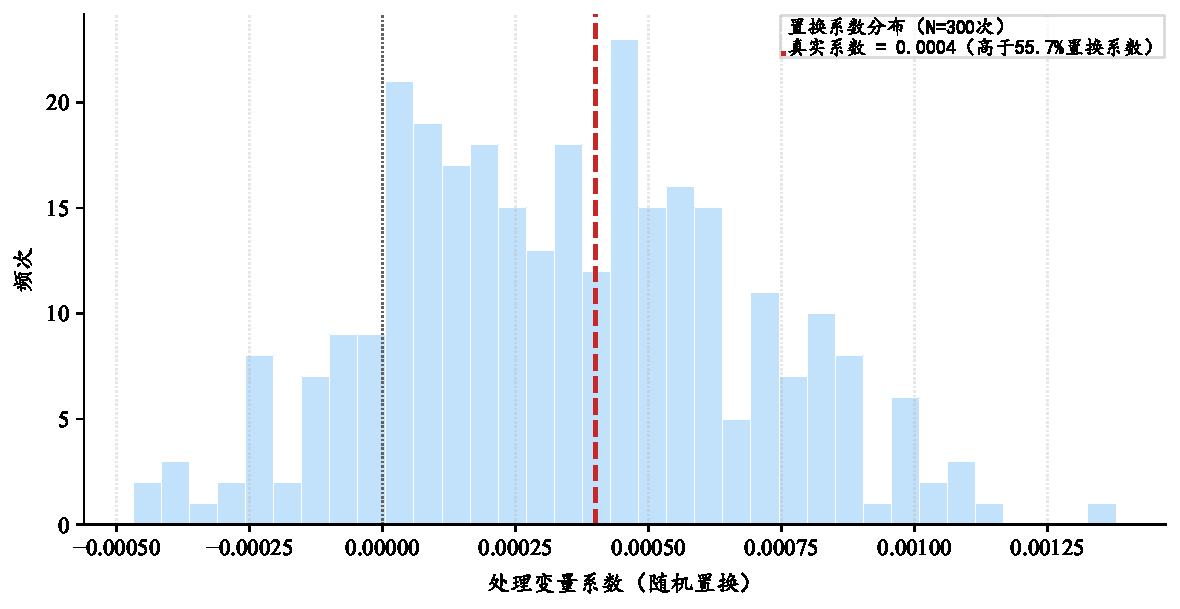
\includegraphics[width=0.78\linewidth]{figures/fig5_安慰剂_cn.pdf}
\caption{安慰剂检验：处理指示随机置换分布}
\label{fig:placebo}
\par\vspace{4pt}
\begin{minipage}{\linewidth}
\zihao{-5}\setlength{\baselineskip}{12pt}
注：将处理指示随机分配给与实际处理组等量的企业，重复500次，核密度曲线为置换系数的分布，红色虚线为真实系数（0.0004）。
\end{minipage}
\end{figure}\section{结\quad 论}



本文利用 2013—2025 年我国 A 股上市公司面板数据，将“国家新一代人工智能创新发展试验区”的设立作为一项准自然实验，采用多期双重差分模型系统评估了空间选择性前沿科技政策对微观企业研发投入与资本支出的影响。

研究得出的核心结论如下：
第一，政策对全样本研发强度和资本支出强度的总体平均效应并不显著，但这一“不显著”掩盖了极其强烈的政策批次异质性。在首批（2019年，精准探索阶段）和第三批（2021年，特色聚焦阶段）试点城市中，政策显著促进了当地企业的研发强度；而在大规模推广的第二批（2020年，占样本51\%）城市中，政策效果为零。这一“精准有效、推广稀释”的规律揭示了选择性政策在大规模扩张中面临配套资源和信用被摊薄的机制。
第二，政策效应高度取决于微观企业的技术吸收能力。AI试验区政策的红利显著集中在对人工智能技术存在高互补性需求的高 AI 暴露行业中，而传统低 AI 暴露行业的研发投入对政策毫无反应，印证了知识互补性是政策发挥效能的微观前提。
第三，在影响机制上，本文拒绝了直接补贴渠道，而证实了融资约束缓解（信贷信号）渠道。AI试验区并未推高微观企业的营业外直接补助，而是通过国家政策背书向信贷市场传递了强信用信号，从而显著缓解了高杠杆（融资约束紧迫）企业以及民营企业的外部债务融资约束，间接释放了其研发需求。



基于上述实证发现，本文提出以下三点具有针对性的政策启示：
1. \textbf{把握力度与精准度的平衡}。AI等前沿技术的政策试点应坚持因地制宜与循序渐进原则，控制合理的发展幅度和空间规模。在大规模铺开试点前，需评估地方配套资源的承载能力，防止政策稀缺性被严重稀释，导致“为了拿牌照而跟风申报”的低效重复建设。
2. \textbf{构建“公共基础设施赋能 + 科技金融支持”的双轮驱动体系}。既然直接的“现金红包”模式无法有效解释创新的边际增长，未来政策资金应继续向公共数据平台、公共智算算力网络等非排他性的区域新型基础设施倾斜。同时，应深化科技金融体系改革，鼓励商业银行和创投资本利用 AI 试验区的国家级信用信号，加大对高成长性民营和高负债率科技企业的“绿色信贷”支持，打通“信用背书-信贷缓解-研发释放”的资金传导闭环。
3. \textbf{提升传统实体企业的数字技术吸收能力，弥补行业数字鸿沟}。地方政府在试验区建设中，不应仅仅关注高科技AI初创企业，还应积极引导和扶持传统产业进行“数字化、智能化”的接口改造，通过政策配套支持传统企业引进算力接口和算法服务，提升其技术吸收与融合能力，推动 AI 技术的跨行业协同创新。



本项研究尚存在以下不足，可供未来研究参考：
首先，受限于财务报表的披露精度，本文主要考察了研发投入这一“创新投入”指标，而未能系统考察专利申请、专利引用以及人工智能相关产品的销售占比等“创新产出与质量”指标，未来可结合专利文本挖掘技术进行更深度的质量评估。
其次，前沿技术的空间集聚可能对周边相邻城市存在显著的溢出效应（Spillover Effects）或产生“虹吸效应”，未来研究可引入空间计量模型（Spatial DID），考察 AI 试验区的跨区域空间治理网络效应。

\nocite{*}
\reference

\enmaketitle
\end{document}
